\documentclass[licencjacka]{pracamgr}
\usepackage[MeX]{polski}
%\usepackage[T1]{fontenc}
\usepackage[utf8]{inputenc}
\usepackage{amssymb}
\usepackage{amsmath}
\usepackage{amsthm}
\usepackage{bbold}
\usepackage{graphicx}
\graphicspath{ {Rysunki/} }
\usepackage[rightcaption]{sidecap}

\theoremstyle{definition}
\newtheorem{definition}{Definicja}[section]

\theoremstyle{definition}
\newtheorem{remark}{Uwaga}[section]

\theoremstyle{definition}
\newtheorem{proposition}{Stwierdzenie}[section]

\theoremstyle{definition}
\newtheorem{example}{Przykład}[section]

\theoremstyle{definition}
\newtheorem{corollary}{Wniosek}[section]

\theoremstyle{plain}
\newtheorem{lemma}{Lemat}[section]

\theoremstyle{plain}
\newtheorem{theorem}{Twierdzenie}[section]

\author{Filip Binkiewicz}

\nralbumu{332069}

\title{Własność A dla kompleksów kostkowych $\text{CAT(0)}$}

\tytulang{Property A for $\text{CAT(0)}$ cube complexes}

\opiekun{prof. dr hab. Sławomira Nowaka\\
			Instytut Matematyki\\
		}

\kierunek{Matematyka}

\date{Czerwiec 2015}

\dziedzina{
11.0 Matematyka, Informatyka:\\
11.1 Matematyka\\
}

\klasyfikacja{14 Algebraic Geometry\\
	}

\keywords{
	Kompleks kostkowy $ \text{CAT(0)} $, własność A
}

\newtheorem{defi}{Definicja}[section]

\def\quotient#1#2{%
    \raise1ex\hbox{$#1$}\Big/\lower1ex\hbox{$#2$}%
}

\begin{document}
\maketitle

%%streszczenie - strona początkowa

\begin{abstract}
%	{
	Praca ta skupia się na dowodzie, iż kompleksy kostkowe $\text{CAT(0)} $
	mają własność A.
%	}
\end{abstract}

\tableofcontents

\chapter*{Motywacja}
\addcontentsline{toc}{chapter}{Motywacja}

Kompleksy kostkowe są pewnym naturalnym uogólnieniem pojęcia grafu na większą liczbę 
wymiarów - zaś własność $ \text{CAT(0)} $ odpowiada za ,,brak cykli'', uogólniając 
analogicznie przypadek szczególny - drzewa. Nie jest 
więc zaskakujące pytanie o ich własności - poniższa praca wprowadza podstawowe 
pojęcia przestrzeni $ \text{CAT(0)} $ oraz kompleksów kostkowych. W poszukiwaniach głębszej 
literatury polecam zajrzeć do \cite{caprace}, \cite{schwer} bądź też \cite{sageev}.

W swojej pracy skupiam się na dowodzie twierdzenia mówiącego, że każdy skończenie 
wymiarowy kompleks kostkowy ma własność $ A $, opierając się na \cite{brodzki}. Własność $ A $, 
po raz pierwszy zdefiniowana przez Yu (więcej informacji w \cite{willett} lub 
\cite{nowak}) 
jest pewnym uogólnieniem pojęcia średniowalności, zdefiniowanym dla grup. Definicja 
nawet optycznie przypomina pewne kryterium średniowalności, a więc istnienie 
ciągu Følnera. Istotne jest to, iż własność $ A $ jest niezmiennikiem relacji 
zgrubnej równoważności, coraz częściej pojawiającej się w literaturze (więcej informacji 
o geometrii zgrubnej można znaleźć w \cite{roe}).

Dowód głównego twierdzenia poparty będzie przykładem, w którym udowodnimy w niestandardowy 
sposób własność $ A $ dla konkretnego kompleksu kostkowego $ \text{CAT(0)} $, 
przestrzeni euklidesowej $ \mathbb{R}^d $. Dalsze postępowanie okaże się równoległe, choć 
nieco bardziej skomplikowane technicznie. 

Jako główny wkład własny w treść pracy traktuję nie treść dowodu głównego twierdzenia, 
zawartego już w \cite{brodzki}, a w który ingerowałem jedynie sporadycznie, przedstawiając 
odrobinę różniące się dowody poszczególnych lematów, lecz rozdział ten dowód poprzedzający. 
Zawarłem w nim zebrane z różnych źródeł definicje, lematy i przykłady dotyczące pojęć 
związanych blisko z tematem mojej pracy, w szczególności własności $ A $, geometrii zgrubnej, 
przestrzeni 
$ \text{CAT(} \kappa \text{)} $ w przypadku szczególnym $ \kappa = 0 $ oraz kompleksów 
kostkowych. 

Dla zainteresowanych starałem się w odpowiednich miejscach pozostawić odnośniki 
do głębszej literatury dotyczącej każdego z tych tematów.


\chapter{Wprowadzenie}

Pierwszy rozdział tej pracy poświęcę przypomnieniu podstawowych definicji, 
twierdzeń i przykładów dotyczących jej tematu. Aby zachować ciągłość pracy, 
postaram się uniknąć przytaczania rozległych dowodów. Dla zainteresowanych 
w odpowiednich miejscach znajdą się odsyłacze do literatury.

\section{Własność A}

Własność A jest pewnym przeniesieniem pojęcia średniowalności na przestrzenie metryczna. 
Przed właściwym wprowadzeniem tego pojęcia przypomnę kilka podstawowych 
definicji dotyczących geometrii zgrubnej.

Przez $ X,Y $ będziemy oznaczać przestrzenie metryczne, $ d $ będzie oznaczać metrykę 
pochodzącą z przestrzeni, z której pochodzą jej argumenty. Jeśli będzie to konieczne, 
przez $ d_X, d_Y $ będziemy dla ścisłości oznaczać metryki pochodzące odpowiednio z $ X $ 
i $ Y $.

\begin{definition}
	Powiemy, że funkcja $ \varphi: X \rightarrow Y $ jest \textbf{zgrubna}, jeśli 
	spełnia następujące dwa warunki:
	\begin{itemize}
	\item (\textit{Bornologiczność}) Dla każdego $ R > 0 $ istnieje $ S > 0 $ 
	takie, że 
	$$ d(x_1,x_2) < R \Rightarrow d \left( \varphi(x_1), \varphi(x_2)\right) < S $$
	\item (\textit{Właściwość}) Dla każdego $ S > 0 $ istnieje $ R > 0 $ takie, że 
	$$ d\left(\varphi(x_1), \varphi(x_2)\right) < S \Rightarrow d(x_1,x_2) < R $$
	\end{itemize}
\end{definition}

\begin{example}
	Zanurzenie $ \mathbb{Z} \hookrightarrow \mathbb{R} $ jest zgrubne. Każde 
	przekształcenie liniowe $ \mathbb{Z} \rightarrow \mathbb{Z}, ~ n \rightarrow
	an + b$ jest zgrubne. Przekształcenie $ \mathbb{Z} \ni n \rightarrow n^2 \in 
	\mathbb{Z} $ nie jest zgrubne, bo nie jest bornologiczne ($ d(n, n+1) = 1 $, a 
	$ d(n^2, n^2 + 2n + 1) = |2n+1| $ jest dowolnie duże).
\end{example}

Powiemy, że dwa przekształcenia $ f_1, f_2 : X \rightarrow Y $ są blisko, 
jeśli istnieje $ C > 0 $ takie, że $$ d(f_1(x), f_2(x)) < C  ~ \text{dla każdego } x \in X$$ 
\begin{definition}
	Powiemy, że przestrzenie $ X,Y $ są \textbf{zgrubnie równoważne}, jeśli 
	istnieją przekształcenia zgrubne $ \varphi : X \rightarrow Y, 
	~ \psi : Y \rightarrow X  $ takie, że 
	$ \varphi \circ \psi $ jest blisko $ \text{id}_Y $, zaś $ \psi \circ \varphi $ jest blisko 
	$ \text{id}_X $.
\end{definition}

\begin{definition}
	Niech $ r > 0$. Powiemy, że
	zbiór $ A \subset X $ jest $ r $-gęsty, jeśli dla każdego $ x \in X $ istnieje 
	element $ a \in A $ taki, że $ d(x,a) < r $. Zbiór $ A $ jest \textbf{zgrubnie gęsty}, 
	jeśli jest $ r $-gęsty dla pewnego $ r > 0 $.
\end{definition}

\begin{remark}
	Każda przestrzeń metryczna $ X $ zawiera dyskretny podzbiór zgrubnie gęsty.
\end{remark}
\begin{proof}
	Ustalmy $ \varepsilon > 0 $. Niech $ \mathcal{D} = \{D \subset X : \forall_{x_1, x_2 \in D, ~
	x_1 \neq x_2} ~ d(x_1, x_2) > \varepsilon \} $. Rodzina $ \mathcal{D} $ jest niepusta 
	oraz każdy łańcuch jest ograniczony z góry przez swoją sumę. Wobec lematu 
	Kuratowskiego-Zorna istnieje więc maksymalny element $D_0 \in \mathcal{D}$. 
	Jest on $ \varepsilon $-gęstym podzbiorem $ X $. 
	Istotnie, załóżmy przeciwnie - istnieje $ x \in X $ taki, że 
	$ d(x, D_0) > \varepsilon $. Wtedy zbiór $ D_0 \cup \{x\} $ należy do rodziny 
	$ \mathcal{D} $ i zawiera w sobie $ D_0 $, co przeczy maksymalności $ D_0 $
\end{proof}

\begin{definition}\label{def:propA}
	Przestrzeń dyskretna $ X $ ma \textbf{własność A}, jeśli dla każdego $ R>0 $ oraz 
	$ \varepsilon > 0 $ istnieje rodzina niepustych, skończonych zbiorów $ A_x \subset 
	X \times \mathbb{N} $ indeksowana $ x \in X $ oraz stała $ S > 0 $ taka, że 
	spełnione są następujące warunki:
	\begin{enumerate}
		\item Dla każdych dwóch $ x,x' \in X $ zachodzi
		$$ d(x,x') < R \Rightarrow \frac{\# (A_x \Delta A_{x'})}{\# A_x} < \varepsilon$$
		\item Dla dowolnego elementu $(x', n) \in A_x$ zachodzi $$ d(x,x') \leq S $$
	\end{enumerate}
	Dowolna przestrzeń metryczna ma własność A, jeśli zawiera zgrubnie gęsty podzbiór 
	o tej własności. Symbol $ \# $ oznacza tu liczbę elementów zbioru, zaś symbol 
	$ \Delta $ - operację różnicy symetrycznej 
	(a więc $A \Delta B = (A \setminus B) \cup (B \setminus A)$)
\end{definition}

\begin{remark}
	Własność A jest niezmiennikiem zgrubnej równoważności przestrzeni dyskretnych. 
	Dokładniej, jeśli przestrzenie dyskretne $ X,Y $ są zgrubnie równoważne, to 
	$ X $ ma własność A wtedy i tylko wtedy, gdy $ Y $ ma własność A.
\end{remark}

Uwaga ta jest bezpośrednią konsekwencją poniższego lematu:

\begin{lemma}
	Jeśli $ \varphi: X \rightarrow Y $ jest przekształceniem zgrubnym przestrzeni dyskretnych 
	oraz $ Y $ ma własność A, to $ X $ ma własność A.
\end{lemma}
\begin{proof}
	Łatwo sprawdzić, że istnieje funkcja $\psi: Y \rightarrow X $ taka, że
	$$ d(y, \varphi(\psi(y)))  \leq d(y,  \varphi(X)) \text{ dla każdego } y \in Y$$
	W tym celu wystarczy dla każdego $ y \in Y $ wybrać $ x \in X $ taki, że 
	$ \varphi(x) $ jest odpowiednio blisko $ y $ i ustalić $ x = \psi(y) $.

	Ustalmy teraz $ R > 0,~  \varepsilon > 0 $. Przekształcenie $\varphi$ jest zgrubne, zatem 
	istnieje $ R_0 $ takie, że $$ d(x,x') < R \Rightarrow d(\varphi(x), \varphi(x')) < R_0 $$ 
	Dla stałych $ R_0, \varepsilon $ istnieje rodzina 
	$ \{B_y \subset Y \times \mathbb{N}\}_{y \in Y} $ 
	indeksowana $ y \in Y $ oraz stała $S'$ spełniającaewarunki definicji własności $ A $.
 	 Zdefiniujmy 
	teraz 
	$$ X \times \mathbb{N} \supset A_x = \{(x', n): ~ n \leq \# \{ (y,m) \in B_{\varphi(x)} : ~
	\psi(y) = x' \}\} $$

	Sprawdzimy, że rodzina ta spełnia warunki definicji \ref{def:propA}. Jeśli 
	$ d(x,x') < R $, to $ d(\varphi(x), \varphi(x')) < R' $, a więc 
	$$ \frac{\# (A_x \Delta A_{x'})}{\# A_x} \leq \frac{\# B_{\varphi(x)} \Delta 
	B_{\varphi(x')}}{\# B_{\varphi(x)}} < \varepsilon $$

	Załóżmy wreszcie, że $ (x', n) \in A_x $. Wówczas istnieje para $ (y,m) \in 
	B_{\varphi(x)} $ taka, że $ \psi(y) = x' $. Wówczas $d(y,\varphi(x)) \leq S'$ oraz 
	$$ d(\varphi(x), \varphi(x')) \leq d(\varphi(x),y) + d(y,\varphi(x')) = d(\varphi(x),y) + 
	d(y, \varphi(\psi(y))) \leq 2S' + 1 $$

	Korzystając znów ze zgrubności $\varphi$, możemy znaleźć stałą $ S $ taką, aby 
	$$ d(\varphi(x), \varphi(x')) < 2S' +1 \Rightarrow d(x,x') < S $$
	Otrzymujemy więc, że $ d(x,x') < S $, co kończy dowód.
\end{proof}

W dalszych rozważaniach będziemy korzystać z następującej charakteryzacji własności A:

\begin{proposition}
	Dyskretna przestrzeń metryczna $ X $ ma własność A wtedy i tylko wtedy, gdy 
	istnieje ciąg rodzin funkcji o skończonym nośniku $ f_{n,x} : X \rightarrow \mathbb{N}
	\cup \{0\} $, indeksowany $ x \in X $, oraz ciąg $ S_n \in \mathbb{R}_{+} $ taki, że
	\begin{enumerate}
		\item Dla każdego $ n $ oraz $ x $ nośnikiem $ f_{n,x} $ jest $ B(S_n, x) $.
		\item Dla każdego $ R > 0 $ ciąg $$ \frac{\| f_{n,x} - f_{n,x'} \|}{\| f_{n,x} \|} $$
		zbiega jednostajnie do zera na zbiorze $ \{ (x,x'): ~ d(x,x') \leq R\} $ przy 
		$ n \rightarrow \infty $. Norma $ \| \cdot \| $ oznacza normę $ \ell_1 $ na 
		przestrzeni funkcji na o skończonym nośniku określonych na $ X $.
	\end{enumerate}
\end{proposition}
\begin{proof}
	Powyższe warunki są równoważne z następującym: dla każdego $ R>0, ~ \varepsilon > 0 $ 
	istnieje rodzina funkcji o skończonym nośniku $ f_x : X \rightarrow \mathbb{N} \cup 
	\{0\}$, indeksowana $ x \in X $, oraz $ S > 0 $ takie, że $ \text{supp}{f_x} = B(S,x)  $ 
	oraz $$ d(x,x') \leq R \Rightarrow \frac{\| f_x - f_{x'} \|}{\|f_x \|} < \varepsilon $$

	Konieczność tego warunku wynika stąd, że przekształcenie $ f_x(y) = \#\left( A_x \cap \left( 
	\{y\} \times \mathbb{N} \right) \right) $ spełnia powyższe warunki, zaś dostateczność - 
	stąd, iż $ A_x = \{(y,n) \in X \times \mathbb{N} : ~ 1 \leq n \leq f_x(y) \} $ spełnia 
	warunki definicji \ref{def:propA}.
\end{proof}

\begin{remark}
	Korzystając z powyższej charakteryzacji w przypadku zbioru wierzchołków kompleksu 
	kostkowego, rozpatrywanego z metryką długości krawędziowej, będziemy 
	sprawdzać warunek drugi jedynie dla stałej $ R = 1 $.
\end{remark}
\begin{proof}
	Niech $ R > 0 $ oraz niech dwa wierzchołki kompleksu $ x $ oraz $ x' $ spełniają 
	$d(x,x') < R $. Istnieje więc $ \mathbb{N} \ni  r < R $ oraz ciąg wierzchołków 
	$ x = x_0, \dots, x_r = x' $, kolejno sąsiednich, stanowiących ścieżkę łączącą 
	$ x $ z $ x' $. Wystarczy wtedy skorzystać z nierówności trojkąta:
	$$ \frac{ \| f_{n,x} - f_{n,x'}\|}{\| f_{n,x}\|} \leq \sum\limits_{i=0}^{r-1}
	\frac{ \| f_{n,x_i} - f_{n,x_{i+1}}\|}{\|f_{n,x}\|} = 
	\sum\limits_{i=0}^{r-1} \frac{ \| f_{n,x_i} - f_{n,x_{i+1}}\|}{\|f_{n,x_i}\|}\cdot
	\frac{\|f_{n,x_i}\|}{\|f_{n,x}\|}$$
	
	Jeśli więc zbieżność ma miejsce na zbiorze sąsiednich wierzchołków, to składnik po 
	prawej stronie również dąży do zera, ponieważ $ \frac{\|f_{n,x}\|}{\|f_{n,x_i}\|} 
	\rightarrow 1$, co wynika stąd, że $ d(x,x_i) < R $ oraz z warunku drugiego.
\end{proof}

\section{Przestrzenie $\text{CAT(0)}$}
Niech $ (X, d) $ będzie przestrzenią metryczną. Odcinkiem geodezyjnym nazywamy 
przekształcenie izometryczne $ \mathbb{R} \supset I \xrightarrow{\rho} X $, gdzie 
$ I =[a,b]$ jest odcinkiem. Przestrzeń $ X $ nazwiemy (jednoznacznie) geodezyjną, 
jeśli każde dwa punkty można połączyć (jednoznacznie wyznaczonym) odcinkiem 
geodezyjnym.

\begin{example}
	Każda przestrzeń euklidesowa $ \mathbb{R}^n $ jest jednoznacznie geodezyjna, 
	jak również każdy jej wypukły podzbiór. Sfera $ S^2 $ jest geodezyjna, ale 
	nie jednoznacznie - dwa bieguny można połączyć ścieżką geodezyjną na 
	nieskończenie wiele sposobów. Każdy spójny graf metryczny jest przestrzenią 
	geodezyjną.
\end{example}

Dalej będziemy rozważać przestrzenie geodezyjne. Dla wygody przez $ [x,y] $ będziemy 
oznaczać (dowolny) odcinek geodezyjny łączący $ x \in X$ z $ y \in X $ (a dokładniej 
obraz tego odcinka).

Zwróćmy uwagę, że jeśli $ X $ jest przestrzenią geodezyjną, to dla każdej trójki 
$ (x,y,z) \in X^3 $ istnieje trójka $ (\overline{x},\overline{y}, \overline{z}) 
\in \left(\mathbb{R}^2\right)^3$ taka, że $ d(x,y) = d_{\mathbb{R}^2} (\overline{x}, 
\overline{y}), ~ d(x,z) = d_{\mathbb{R}^2} (\overline{x}, \overline{z}), 
~ d(y,z) = d_{\mathbb{R}^2} (\overline{y}, \overline{z})  $. Innymi słowy, każdemu 
trójkątowi z $ X $ można przypisać trójkąt z przestrzeni euklidesowej $ \mathbb{R}^2 $ o 
bokach takiej samej długości. Taki trójkąt jest wyznaczony jednoznacznie z dokładnością 
do izometrii przestrzeni $ \mathbb{R}^2 $ i nazwiemy go trójkątem porównania $ (x,y,z) $.

\begin{definition}
	Powiemy, że przestrzeń geodezyjna $ X $ jest $ \text{\textbf{CAT(0)}} $, jeśli 
	dla każdej trójki $ (x,y,z) \in X^3 $ oraz punktu $ p \in [y,z] $ oraz odpowiadającym 
	im trójkątowi porównania $ (\overline{x}, \overline{y}, \overline{z}) \in 
	\left(\mathbb{R}^2\right)^3 $ i punktowi $ \overline{p} \in [\overline{y}, 
	\overline{z}] $ zachodzi nierówność:
	$$ d(x,p) \leq d_{\mathbb{R}^2}(\overline{x}, \overline{p}) $$
\end{definition} 
\begin{SCfigure}[0.7][h]
	\caption{\small{Intuicyjnie, trójkąty w przestrzeniach $ \text{CAT(0)} $ są ,,szczuplejsze''
	niż w przestrzeni euklidesowej.}}
	\centering
	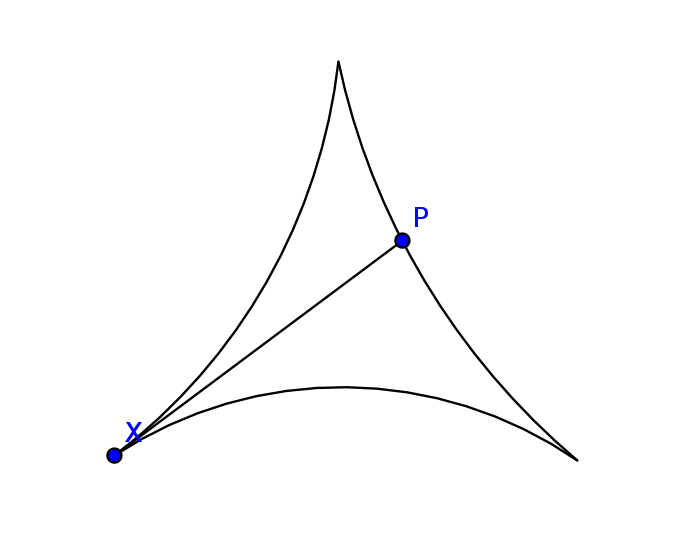
\includegraphics{trojkat_hiperboliczny}
%%miejsce na rysuneczek chudego trójkąta
\end{SCfigure}

\begin{example} Nietrudno jest o kilka przykładów takich przestrzeni:
	\begin{itemize}
	\item Każda przestrzeń euklidesowa $ \mathbb{R}^n $ jest $ \text{CAT(0)} $. Wówczas 
	wymieniona nierówność jest po prostu równością.
	\item Graf metryczny jest przestrzenią $ \text{CAT(0)} $ wtedy i tylko wtedy, gdy 
	jest drzewem.
	\end{itemize}
\end{example}

\begin{remark}
	Każda przestrzeń $ \text{CAT(0)} $ jest jednoznacznie geodezyjna.
\end{remark}
\begin{proof}
	Przypuśćmy przeciwnie i niech $ x,y \in X $ łączą dwa różne odcinki geodezyjne, 
	powiedzmy $ [x,y], \overline{[x,y]} $.	Wówczas istnieją $ [x,y] \ni p \neq \overline p 
	\in	\overline{[x,y]}  $ takie, że $ d(x,p) = d(x,\overline{p}) $ oraz $ d(y,p) = 
	d(y, \overline{p}) $. Wówczas trójkątowi $ (x,y,\overline{p}) $ w $ \mathbb{R}^2$ 
	odpowiada trójkąt zdegenerowany, zaś $ d(p,\overline{p}) > 0 $, co przeczy nierówności 
	$ \text{CAT(0)} $
\end{proof}

\begin{corollary}
	Sfera $ S^2 $ nie jest przestrzenią $ \text{CAT(0)} $. Płaszczyzna $ \mathbb{R}^2 $ 
	wyposażona w metrykę pochodzącą od normy $ \ell_1 $ nie jest przestrzenią $ \text{CAT(0)} $
	\begin{SCfigure}
	\caption{\small{Na rysunku zaznaczono dwa odcinki geodezyjne łączące punkty 
	$ x = (0,0) $ i $ x_1 = (1,1) $ na płaszyźnie z metryką pochodzącą od normy $ \ell_1 $}}
	\centering
	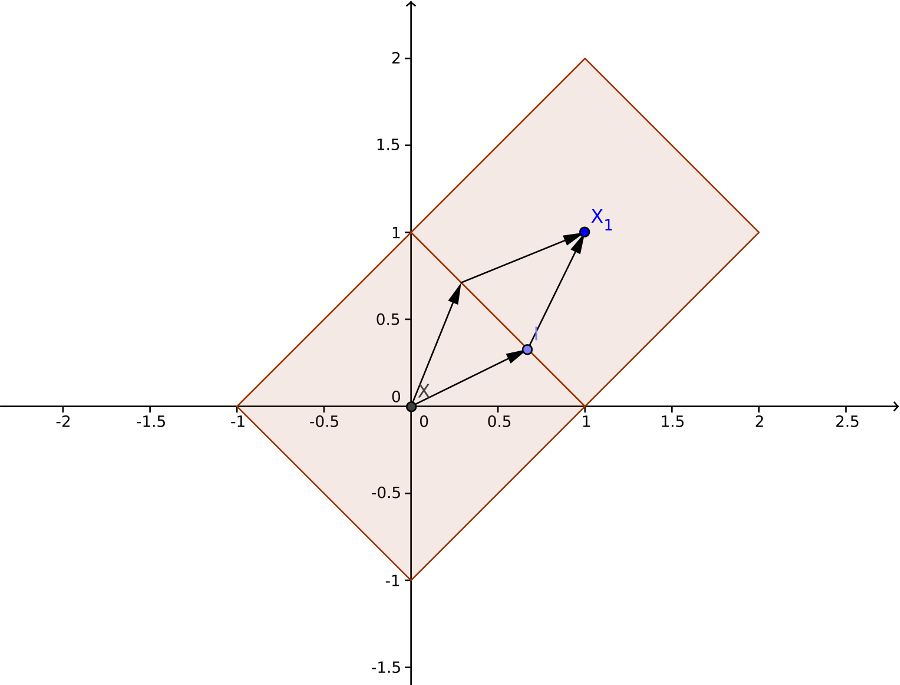
\includegraphics{plaszczyzna_l1}
	\end{SCfigure}
\end{corollary}

\section{Kompleksy kostkowe $ \text{CAT(0)} $}
Niech $ K = [0,1]^n $ będzie $ n $-wymiarową kostką. Będzie to podstawowy ,,budulec'' 
interesujących nas przestrzeni. Przez ścianę o kowymiarze równym 1 będziemy rozumieć zbiór 
$$ F_{i,\varepsilon}  = \{x \in K : ~ x_i = \varepsilon\}, ~ \text{ dla } i = 1 
\dots n \text{ oraz }\varepsilon \in \{0,1\}$$

Wszystkie ściany o niższym kowymiarze (o wyższym wymiarze) można otrzymać jako 
przecięcie ścian o wyższym kowymiarze.

\begin{definition}
	Niech $ K,K' $ będą dwiema kostkami oraz $ F \subset K, ~ F' \subset K' $ będą 
	ich ścianami. \textbf{Sklejeniem} (lub \textbf{przyłączeniem}) $ K $ z $ K' $ nazwiemy 
	izometrię $ \varphi: F \rightarrow F' $.
\end{definition}

\begin{definition}
	Przypuśćmy, że $ \mathcal{K} $ jest zbiorem kostek (dla każdego $ K \in 
	\mathcal{K} $ istnieje $ n(K) \in \mathbb{N} $ takie, że $ K \simeq [0,1]^{n(K)} $), 
	zaś $ \mathcal{S} $ - zbiorem sklejeń elementów $ \mathcal{K} $ (każdemu 
	$ \varphi \in \mathcal{S} $ odpowiadają kostki $ K = K(\varphi), K' = 
	K'(\varphi) \in \mathcal{K} $ oraz ściany $ F \subset K, F' \subset K' $. Załóżmy 
	wreszcie, że taka para 	$ (\mathcal{K}, \mathcal{S})  $ spełnia następujące warunki:

	\begin{enumerate}
		\item Żadna kostka nie jest sklejona sama ze sobą.
		\item Dla każdych dwóch kostek $ K \neq K' $ istnieje co najwyżej jedno
		sklejenie $ K $ z $ K'$.
	\end{enumerate}

	Wówczas w następujący sposób można zdefiniować \textbf{kompleks kostkowy}:
	$$ X =  \quotient{\left( \bigsqcup\limits_{K \in \mathcal{K}} C \right)}{\sim} $$

	gdzie $ \sim $ dla każdego $ \varphi \in \mathcal{S} $ utożsamia dziedzinę $ \varphi $ 
	z jego obrazem, to znaczy: $$ \{ x \sim \varphi(x) ~ | ~ \varphi \in \mathcal{S}, ~ 
	x \in \text{dom}(\varphi) \} $$

	Jeśli istnieje stała $ M > 0 $ taka, że dla każdego $  K  \simeq [0,1]^{n(K)}\in 
	\mathcal{K} $ zachodzi $ n(K) < M $, to kompleks kostkowy $ X $ jest \textbf{skończenie 
	wymiarowy}. Wtedy \textbf{wymiarem} tego kompleksu nazwiemy liczbę 
	$$ \dim X = \max\limits_{K \in \mathcal{K}} n(K)$$
\end{definition}

\begin{remark}
	W ten sposób zdefiniowany kompleks kostkowy jest przestrzenią metryczną, przy czym 
	metryka długości indukowana jest z metryki euklidesowej 
	na $ [0,1]^n \subset \mathbb{R}^n$. Odległość punktów $ x,y $ mierzona w metryce 
	długości jest to infinum długości krzywych $ \gamma : [a,b] \rightarrow X $ 
	łączących $ x$ z $ y $. Długość krzywej definiujemy następująco: 
	$$ l(\gamma) = \sup\limits_{a = t_0 \leq \dots \leq t_n = b} \sum\limits_{i=0}^{n-1}
	d(\gamma(t_i), \gamma(t_{i+1})) $$
\end{remark}
\begin{proposition}
	Z powyższej definicji łatwo wynikają następujące fakty:
	\begin{itemize}
	\item Obcięcie rzutowania $ p : \bigsqcup_{K \in \mathcal{K}} K \rightarrow X$ do jednej 
	kostki $ K \in \mathcal{K}$ jest iniekcją.
	\item Niepuste przecięcie dwóch kostek jest ścianą obydwu.
	\end{itemize}	
\end{proposition}

\begin{example}
	Łatwo o kilka prostych przykładów kompleksów kostkowych:
	\begin{itemize}
	\item Rozważmy graf metryczny bez wierzchołków izolowanych, w którym każda krawędź ma 
	długość 1. Każda krawędź jest izometryczna z $ [0,1] $, zaś sklejenia to
	po prostu izometrie punktów.
	\item Torus można interpretować jako kompleks kostkowy. Rozważmy zbiór 
	$ [0,3]\times[0,3] \subset \mathbb{R}^2 $, w którym można wprowadzić podział 
	na dziewięć części izometrycznych z $ [0,1]^2 $. Wtedy odpowiednie izometrie 
	prowadzą do konstrukcji torusa (rysunek).
	%miejsce na rysuneczek torusa
	\begin{SCfigure}[0.8][h]
	\caption{\small{Klasyczna konstrukcja torusa jako przykład kompleksu kostkowego. 
	Strzałki wyznaczają izometrie odpowiednich krawędzi}}
	\centering
	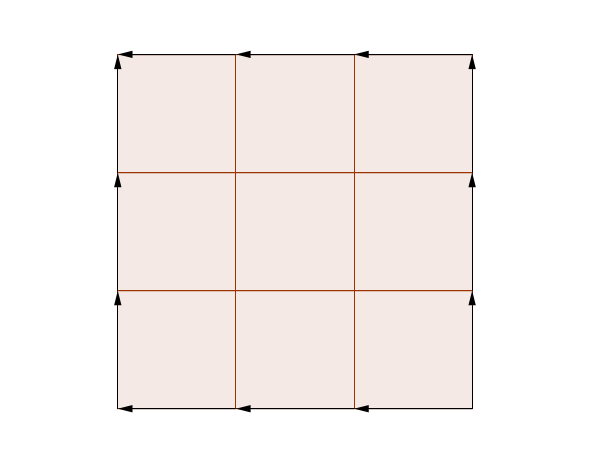
\includegraphics{torus}
	\end{SCfigure}
	\end{itemize}
\end{example}


\begin{remark}
	Na zbiorze wierzchołków kompleksu kostkowego można wprowadzić metrykę 
	długości krawędziowej, według której 
	odległość dwóch wierzchołków to minimum długości łączących ich ścieżek złożonych 
	z krawędzi kompleksu (przez krawędź rozumiemy ścianę o wymiarze 1).
	Z naszego punktu widzenia możemy utożsamić te metryki, z uwagi na następujący fakt:
\end{remark}

\begin{proposition}
	Niech $ X $ będzie kompleksem kostkowym $ \text{CAT(0)}$. Metryka długości na 
	zbiorze wierzchołków $ X $ jest zgrubnie równoważna z metryką długości krawędziowej.
	Jeśli $ X $ jest skończenie wymiarowy, to zbiór wierzchołków z pierwszą bądź drugą z 
	tych metryk jest sobie zgrubnie równoważny.
\end{proposition}
\begin{proof}
	Identyczność jest zgrubną równoważnością.
\end{proof}

\begin{definition}
	Niech $ K \simeq [0,1]^n $ będzie kostką. Wówczas \textbf{śródkostką} $ K $ nazwiemy 
	zbiór
	$$ M_i = \{ x \in K : x_i = 1/2 \} \text{ dla } i = 1,\dots,n $$
\end{definition}
Wprowadźmy na chwilę następującą relację równoważności: dwie krawędzie w kompleksie 
kostkowym są sobie \textbf{kwadratowo równoważne} (piszemy: $ e \sim e' $), jeśli 
są sobie naprzeciwległe w pewnym kwadracie w tym kompleksie. Taką relację rozszerzamy do 
relacji równoważności.
\begin{definition}
	\textbf{Hiperpłaszczyzną} dualną do klasy równoważności $ [e] $ (lub po prostu do 
	krawędzi $ e $) nazwiemy sumę śródkostek przecinających elementy klasy $ [e] $.
\end{definition}

\begin{SCfigure}[0.8][h]
	\caption{\small{Przykład hiperpłaszczyzny w kompleksie kostkowym. Ciemniejszym kolorem
	zaznaczono hiperpłaszczyznę dualną do krawędzi E}}
	\centering
	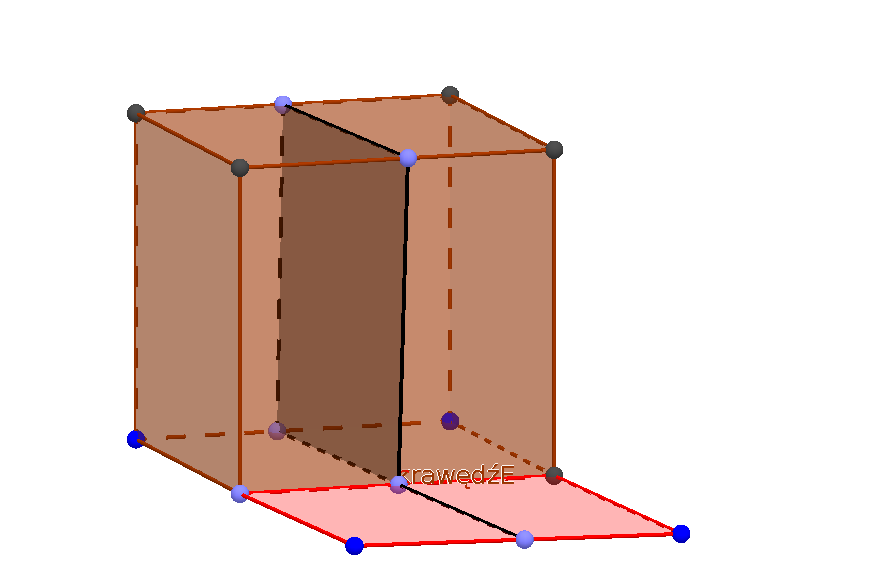
\includegraphics{hiper}
\end{SCfigure}

Zwróćmy uwagę, że hiperpłaszczyzna wyznacza podział zbioru wierzchołków na dwa 
podzbiory, które będziemy dalej nazywać \textbf{półpłaszczyznami}. 
Będzie to miało kluczowe znaczenie kombinatoryczne. 
Dwie hiperpłaszczyzny tworzą podział kompleksu na cztery przecięcia półpłaszczyzn. Jeśli 
wszystkie są niepuste, to hiperpłaszczyzny \textbf{przecinają się}. Dwa wierzchołki 
$ x,y $ są \textbf{oddzielone} przez hiperpłaszczyznę $ H $, jeśli należą do różnych 
wyznaczonych przez nią półprzestrzeni. 

\begin{remark}
	Zgodnie z definicją \ref{def:propA} przestrzeń metryczna ma własność $ A $, jeśli 
	zawiera dyskretną podprzestrzeń, która ma tę własność. Oczywiście w przypadku kompleksów 
	kostkowych szukaną podprzestrzenią jest przestrzeń wierzchołków. Dlatego też w dalszej 
	części pracy przez $ X $ będziemy oznaczać zbiór \underline{wierzchołków} 
	kompleksu kostkowego, zaś przez $ x, x', y, z $ - wierzchołki. \textbf{Kompleksem 
	kostkowym CAT(0)} nazwiemy oczywiście kompleks kostkowy, który jest dodatkowo 
	$ \text{CAT(0)} $. 
\end{remark}

Zbiór hiperpłaszczyzn oddzielających $ x $ od $ y $ będziemy oznaczać przez 
$\mathfrak{H}(x,y)$. \textbf{Odcinkiem} łączącym $ x $ oraz $ y $ nazwiemy przecięcie 
wszystkich półprzestrzeni zawierających obydwa te punkty i oznaczymy $ [x,y]$. Zbiór 
wierzchołków $ V $ nazwiemy \textbf{wypukłym}, jeśli dla każdych $ x,y \in V $ również 
$ [x,y] \subset V $.

Dla trzech wierzchołków $ w,x,y $ możemy wyróżnić ich \textbf{medianę}, zdefiniowaną 
jako jedyny wierzchołek należący do $ [w,x] \cap [x,y] \cap [w,y] $

Dla kompleksu kostkowego $ \text{CAT(0)}~ X$ możemy wprowadzić brzeg kombinatoryczny. 
Niech funkcja $ \sigma $ przypisuje hiperpłaszczyźnie $ X $ jedną z wyznaczonych przez nią 
półprzestrzeni, przy czym dla każdych dwóch hiperpłaszczyzn $ H_1, H_2 $ zachodzi 
$ \sigma(H_1) \cap \sigma(H_2) \neq \emptyset $. Taką funkcję nazwiemy \textbf{ultrafiltrem}.

Wierzchołek $ x $ definiuje takie przekształcenie: dla hiperpłaszczyzny $ H $ wyznacza 
półprzestrzeń $ H_x $ zawierającą $ x $ (rzeczywiście, dla każdych dwóch hiperpłaszczyzn 
$ H,K $ mamy $ x \in H \cap K $). Jeśli więc oznaczymy przez $\mathfrak{U}$ zbiór wszystkich 
ultrafiltrów na $ X $ to wskazaliśmy iniekcję 
$$ \iota : X \rightarrow \mathfrak{U} $$

Wówczas elementy zbioru $$ \partial X = \mathfrak{U} \setminus \iota(X) $$
nazwiemy \textbf{krawędziami w nieskończoności}. Utożsamiając z wierzchołkiem $ x $ 
ultrafiltr $ \iota(x) $, możemy więc zdefiniować
$$ \overline{X} = X \cup \partial X $$
Powyższy zbiór nazwiemy \textbf{dopełnieniem w nieskończoności} kompleksu $ X $.

Możemy przenieść podstawowe kombinatoryczne własności 
kompleksu kostkowego $ \text{CAT(0)}$ 
na jego dopełnienie w nieskończoności. Jeśli $ z,w \in \overline{X} $, to dla 
hiperpłaszczyzny $ H $ przez $ H_z, H_w $ będziemy oznaczać obraz $ z,w $ 
(jako ultrafiltrów) na 
$ H $, a więc odpowiednią półprzestrzeń (wtedy powiemy, że $ H_z $ zawiera $ z $. 
Hiperpłaszczyzna $ H $ \textbf{oddziela} $ x $ od $ w $, 
jeśli $ H_z \neq H_w $. Można więc na $ \overline{X} $ uogólnić definicję zbioru 
$ \mathfrak{H}(x,w)$. Podobnie możemy zdefiniować odcinek $ [x,w] $ jako 
$$ [x,w] = \bigcap H_{x,w}  ~~ x,w \in H_{x,w}, ~ H_{x,w} - \text{ półprzestrzeń}$$

Zwróćmy uwagę, że każdy odcinek $ [x,w] $ jest wypukły. Wynika to stąd, że przecięcie 
zbiorów wypukłych takie jest. Oczywiste jest również następujące stwierdzenie: 

\begin{proposition}
	Niech $ x,y,w \in X $ oraz $ x \in \overline{X} $. Jeśli $ w \in [x,z] $ oraz 
	$ y \in [y,w] $, to $ \mathfrak{H}(y,w) \subset \mathfrak{H}(y,z)$
\end{proposition}

\begin{remark}
	Na zbiorze $ \overline{X} $ trudno wprowadzić metrykę, można natomiast w naturalny 
	sposób zrobić z niego przestrzeń topologiczną. Powiemy, że ciąg wierzchołków 
	$ \{x_j\}_{j = 1}^{\infty} \subset X $ zbiega do wierzchołka $ x \in \overline{X} $, jeśli 
	dla każdej hiperpłaszczyzny $ H $ zachodzi $ H \in \mathfrak{H}(x_j, x) $ jedynie 
	dla skończenie wielu $ j $. Piszemy wówczas, że $$ x_j 
	\xrightarrow{j \rightarrow \infty} x $$
\end{remark}

Sekcję tę zakończymy serią lematów i twierdzeniem łączącym kompleks 
kostkowy z przestrzenią euklidesową.

\begin{lemma}
	Niech $ \{x_j\}_{j = 1}^{\infty} \subset X, x \in \overline{x} $ oraz niech 
	$ x_j \rightarrow x$ przy $ j \rightarrow \infty $. Hiperpłaszczyzna $ H $ 
	oddziela $ y $ od $ x $ wtedy i tylko wtedy, gdy oddziela $ y $ od prawie 
	wszystkich\footnote{wszystkich, oprócz skończenie wielu} $ x_j $. Inaczej:
	$$ \mathfrak{H}(y,x) = \bigcup\limits_{k = 1}^{\infty} \bigcap\limits_{j = k}^{\infty}
	\mathfrak{H}(y,x_j) $$
\end{lemma}
\begin{proof}
	Wystarczy wspomnieć definicję: $ H $ oddziela $ y $ od $ x $ wtedy i tylko wtedy, gdy 
	$ H_y \neq H_z $, a więc wtedy i tylko wtedy, gdy $H_y \neq H_{x_j} $ dla prawie 
	wszystkich $ j \in \mathbb{N} $. 
\end{proof}
\begin{lemma}
	Niech $ \{x_j\}_{j = 1}^{\infty} \subset X, x \in \overline{X} $ oraz niech 
	$ x_j \rightarrow x$ przy $ j \rightarrow \infty $. Ponadto niech $ y,z \in X $. 
	Wówczas jeden \underline{i tylko jeden} z poniższych warunków jest prawdziwy.
	\begin{itemize}
		\item $ y \in [z,x_j] $ dla prawie wszystkich $ j \in \mathbb{N} $
		(wtedy $ y \in [z,x]$).
		\item $ y \notin [z,x_j] $ dla prawie wszystkich $ j \in \mathbb{N} $
		(wtedy $ y \notin [z,x] $).
	\end{itemize}
\end{lemma}
\begin{proof}
	Negacją warunku pierwszego jest warunek: $ y \notin [z,x_j] $ dla nieskończenie 
	wielu $ j \in \mathbb{N} $. Wynika on łatwo z drugiego warunku. Pokażemy, że warunek 
	drugi jest mu równoważny.
	
	Jeśl $ y \notin [z,x_j]  $, to istnieje $ H \in \mathfrak{H}(y,z) $ taka, że 
	$ H_z = H_{x_j} $. %%whyyyyyyy.
	Jeśli jest tak dla nieskończenie wielu $ j $, to ze skończoności zbioru 
	$ \mathfrak{H}(y,z) $ wynika, że istnieje hiperpłaszczyzna 
	$ H \in \mathfrak{H}(y,z)$ taka, że $ H_{z} = H_{x_j} $ dla nieskończenie wielu $ j \in 
	\mathbb{N} $. Zatem $ H_z = H_x = H_{x_j} $ dla prawie wszystkich $ j \in \mathbb{N} $. 
	W szczególności $ y \notin [z,x_j] $ dla niemal wszystkich $ j $, a więc 
	$ y \notin [z,x] $.
	
	Pozostaje wykazać, że pierwszy warunek pociąga za sobą, że $ y \in [z,x] $.
	Załóżmy że $ y \notin [z,x] $. Istnieje więc hiperpłaszczyzna  
	$ H \in \mathfrak{H}(y,z) $ taka, że $ H_x = H_z $, a więc $ H_{x_j} = H_{z} $ dla 
	niemal wszystkich $ j \in \mathbb{N} $. A więc $ y \notin [z,x_j] $ dla 
	prawie wszystkich $ j \in \mathbb{N} $ i otrzymujemy sprzeczność.
\end{proof}

\begin{lemma}
	Niech $ x,y \in X $ oraz $ z \in \overline{X} $. Wówczas przecięcie odcinków 
	$ [x,y], [x,z], [y,z] $ składa się z pojedynczego wierzchołka z $ X $.
\end{lemma}
\begin{proof}
	Najpierw wykażemy, że przecięcie to jest niepuste, następnie - że ma tylko jeden element.

	Niech $ \{z_j\}_{j = 1}^{\infty} \subset X $ będzie ciągiem wierzchołków zbieżnym 
	do $ z $. Odcinek $[x,y] $ jest skończony i zawiera mediany $ m_j = m(x,y,z_j) $. 
	Istnieje więc $ m \in [x,y] $ taki, że $ m = m_j \in [x,z_j] $ dla nieskończenie 
	wielu $ j \in \mathbb{N} $. Z poprzedniego lematu wynika więc, że $ m \in [x,z_j] $ dla 
	niemal wszystkich $ j \in \mathbb{N} $ oraz $ m \in [x,z] $. Podobnie $ m \in [y,z] $.

	Załóżmy teraz, że $ m \neq m' $ należą do $ [x,y] \cap [x,z] \cap [y,z] $ i niech 
	$ H \in \mathfrak{H}(m,m') $. Któreś dwie z półprzestrzenie $ H_x, H_y, H_z $ są 
	sobie równe; dla ustalenia uwagi niech $ H_x = H_y $. Skoro $ H_m \neq H_{m'} $, 
	tylko jedno z nich może być równe $ H_x $, zatem znowu dla ustalenia uwagi niech 
	$ H_m \neq H_x $. Wtedy $ m \notin [x,z] $, co daje sprzeczność.
\end{proof}

\begin{remark}
	W powyższym dowodzie skorzystaliśmy z faktu, że mamy ciąg $X \ni z_j \rightarrow z \in 
	\overline{X}$. 
	Istnienie takiego ciągu nie jest zupełnie oczywiste - aby je uzasadnić, należy 
	rozważyć zbiór wszystkich hiperpłaszczyzn $ H_1, H_2, \dots $ (jest on przeliczalny) 
	oraz dla każdego $ j \in \mathbb{N}$ wybrać $ z_j $ należące do zbioru
	$$ \bigcap\limits_{i=1}^j (H_i)_z $$
	
	Aby uzasadnić, że powyższy zbiór jest niepusty, wystarczy skorzystać z twierdzenia 
	Helly'ego mówiącego o przecięciach zbiorów wypukłych (patrz \cite{helly}). 
	%rol98, Helly's theorem
\end{remark}
Dla $ x \in X, z \in \overline{X} $ przez $ \mathfrak{R}_z(x) $ oznaczymy 
podzbiór $ \mathfrak{H}(x,z) $ złożony z tych hiperpłaszczyzn, które oddzielają 
$x $ od $ z $ oraz pewnego sąsiada $ x $. 
\begin{lemma}
	Niech $ X $ będzie kompleksem kostkowym $ \text{CAT(0)} $ oraz $ \dim{X} < \infty $. 
	Ponadto niech $ x \in X, z \in \overline{X} $.
	Wówczas $ \# \mathfrak{R}_z(x) \leq \dim{X}$
\end{lemma}
\begin{proof}
	Dowód można znaleźć w \cite{brodzki}, lemat 1.13
\end{proof}

W następnym twierdzeniu uzasadnimy, że odcinki łączące wierzchołki (być może 
w nieskończoności) zanurzają się w odpowiednio dużą przestrzeń euklidesową. W oczywisty 
sposób $ \mathbb{R}^d $ możemy postrzegać jako kompleks kostkowy (patrz przykład 1.3.1). 
Zbiorem wierzchołków jest krata $ \mathbb{Z}^d $. Odcinkami są prostopadłościany - 
dokładniej, jeśli 
$ \overline{x} = (x_1, \dots, x_d), \overline{y} = (y_1, \dots, y_d)  \in\mathbb{Z}^d $, 
to odcinkiem $ [\overline{x}, \overline{y}] $ jest powłoka wypukła podzbioru $ \mathbb{Z}^d$ 
złożonego z tych liczb, których $ i $-ta współrzędna jest z przedziału $ [x_i, y_i] $ lub
$ [y_i, x_i] $.
Żeby włączyć do naszych rozważań wierzchołki w nieskończoności, dopuszczamy możliwość, że 
$ x_i  $ lub $ y_i = \pm \infty $ dla pewnego $ i = 1 \dots d$.

\begin{theorem} \label{thm:zanurzanie}
	Niech $ X $ będzie skończenie wymiarowym kompleksem kostkowym $ \text{CAT(0)} $, 
	$ \dim{X} = d $ oraz niech $ x,y \in \overline{X} $. Wówczas odcinek $ [x,y] $ zanurza 
	się izometrycznie w kompleksie kostkowym $ \mathbb{R}^d $.
\end{theorem}

Wprowadźmy na zbiorze $ \mathfrak{H}(x,y) $ częściowy porządek w następujący sposób:
$$ H \preceq K \iff H_x \subset K_x $$

\begin{lemma}
	Dwie płaszczyzny $H,K \in \mathfrak{H}(x,y)$ nie są porównywalne w tym 
	porządku wtedy i tylko wtedy, gdy się przecinają.
\end{lemma}
\begin{proof}
	Oczywiste jest, że $ H_x \cap K_x \neq \emptyset \neq H_y \cap K_y $. Dalej, 
	$ H_x \cap K_y = \emptyset \iff H_x \subset K_x  \wedge H_y \cap K_x = \emptyset \iff
	K_x \subset H_x$. $ H $ oraz $ K $ są więc nieporównywalne przez $ \preceq $ wtedy 
	i tylko wtedy, gdy $ K_x \not\subset H_x $ oraz $ H_x \not\subset K_x $, a więc 
	wtedy, gdy wszystkie cztery przecięcia są niepuste.
\end{proof}

\begin{lemma}[Dilworth]
	Niech $ (S, \preceq) $ będzie zbiorem częściowo uporządkowanym. Łańcuchem nazwiemy 
	podzbiór $S $, 
	którego elementy są parami porównywalne, antyłańcuchem - podzbiór $ S $ nieposiadający 
	dwóch różnych elementów porównywalnych. Jeśli zbiór $ S $ nie zawiera antyłańcucha 
	o mocy $ m + 1 $, to $ S $ jest sumą rozłączną $ m $ łańcuchów.
\end{lemma}
\begin{proof}
	Można znaleźć w (Dilworth, a decomposition theorem for partially ordered sets).
\end{proof}
\begin{corollary}
	Zbiór częściowo uporządkowany $ \left(\mathfrak{H}(x,y), \preceq \right) $ 
	jest sumą rozłączną $ d $ 
	łańcuchów.	
\end{corollary}
\begin{proof}
	Wystarczy skorzystać z twierdzenia Helly'ego, lematu Dilwortha oraz 
	lematu 1.3.5 
\end{proof}
\begin{proof}[Dowód twierdzenia 1.3.1]
	Dowód tego twierdzenia przeprowadzimy tylko dla przypadku, gdy $ x $ jest 
	wierzchołkiem $ X $. Weźmy rozkład zbioru $ \mathfrak{H}(x,y)$ na łańcuchy, którego 
	istnienia dostarcza poprzedni lemat
	 $$ \mathfrak{H}(x,y) = \bigsqcup\limits_{i=1}^{d} \mathfrak{B}_i  $$
	Niech teraz 
	$$ X \supset [x,y] \ni z \rightarrow \overline{z} = (\overline{z_1}, \dots, 
	\overline{z_d}) \in \mathbb{Z}^d, ~ \overline{z_i} = \# \{H \in \mathfrak{B}_i: ~ 
	z \in H_y\} $$

	Wówczas $ \overline{x} = 0$, zaś $ \overline{y} = (\overline{y_1}, \dots, 
	\overline{y_d}) $, gdzie $ \overline{y_i} = \# \mathfrak{B}_i, i = 1 \dots d$. 
	Dla każdego $ z \in [x,y] $ współrzędne $ \overline{z} $ są skończone oraz 
	$ \overline{z} \in [\overline{x}, \overline{y}] $.

	Funkcja $ z \rightarrow \overline{z} $ zanurzeniem izometrycznym. Żeby to sprawdzić, 
	wystarczy obliczyć:
	$$ d(\overline{v}, \overline{w}) = \sum\limits_{i=1}^d \# \{ 
	H \in \mathfrak{B}_i: ~ H \in \mathfrak{H}(v,w) \} = \# \mathfrak{H}(v,w) = 
	d(v,w)$$
\end{proof}

\section{Kombinacje}
Funkcje, spełniające warunki Stwierdzenia 1.1.1. będziemy konstruować przy 
użyciu dwumianu Newtona, a więc funkcji $ {n \choose k} $. Kombinatorycznie funkcja ta 
oznacza \textit{liczbę $ k $-podzbiorów $ n $-zbioru}, w szczególności jej definicja jest 
poprawna dla całkowitych $ n \geq k \geq 0 $. Przy użyciu łatwej interpretacji 
kombinatorycznej można udowodnić relację rekurencyjną:

\begin{itemize}
	\item $ {n \choose 0} = {n \choose n} = 1 $ dla $ n \geq 0 $.
	\item $ {n \choose k} = {n-1 \choose k-1} + {n-1 \choose k} $
\end{itemize}

Można łatwo uogólnić tę funkcję dla wszystkich $ n,k \in \mathbb{Z} $ poprzez relację:

\begin{itemize}
	\item $ {n \choose 0} = 1  $ dla $ n \geq 0$ oraz $ {n \choose n} = 1  $ dla 
	$ n \in \mathbb{Z}$
	\item $ {n \choose k} = {n -1 \choose k-1} + {n-1 \choose k} $ dla wszystkich $ n,k \in
	\mathbb{Z} $
\end{itemize}

Z powyższej definicji łatwo udowodnić kilka własności:

\begin{itemize}
	\item ${n \choose k} = 0$ dla $ k < 0 \leq n $
	\item $ {n \choose k} = (-1)^{n+k}{-1-r \choose -1-n} $
\end{itemize}

Szczególnie przydatna okaże się druga własność, dla $ k = -1 $. Przyjmuje wtedy ona formę 
$$ {n \choose -1} = (-1)^{n-1} {0 \choose -1-n} $$

\chapter{Kompleksy kostkowe $ \text{CAT(0)} $ a własność A}

W tym rozdziale skupimy się na dowodzie twierdzenia łączącego kompleksy kostkowe 
$ \text{CAT(0)} $ z własnością A. Zaczniemy od przykładu motywującego dowód głównego 
twierdzenia. O funkcjach $ f_{n,x} $ wymienionych w Stwierdzeniu 1.1.1. będziemy mówić jako o 
\textit{funkcjach wagowych}. Również z warunków podanych w tym stwierdzeniu korzystać 
będziemy zamiast definicji własności $A$.

Ustalmy również pewien wymiar $\mathbb{N} \ni N \geq d $. 
Niektóre lematy prawdziwe będą również dla przypadku $ N = d-1$ - zostanie to odpowiednio 
podkreślone.

\section{Własność $ A $ dla przestrzeni euklidesowych}

\begin{example}
	Niech $ T $ będzie $ \mathbb{R} $-drzewem, a więc spójnym grafem niezawierającym cykli. 
	Aby pokazać, że $ T $ ma własność $ A $, ustalmy korzeń $ K $. Dla każdego wierzchołka 
	$ x \in X $ oraz $ n \in\mathbb{N} $ definiujemy funkcję wagową
	$$ \tilde f_{n,x}(y) = 
	\begin{cases}
		1 & \text{ jeśli } y \neq K \\
		n - d(x,y) & \text{ jeśli } y = K
	\end{cases} $$
	Wówczas ciąg rodzin funkcji $ f_{n,x}(y) = \tilde f_{n,x}(y) \cdot \mathbb{1}_{B
	(x, n)} (y) $ spełnia warunki Stwierdzenia 1.1.1
\end{example}

Pewna intuicja stojąca za tym przykładem jest następująca: przy $ n $ dążącym do 
nieskończoności rozkładamy wagę równomiernie na kuli $ B(x,n) $, nadmiar zrzucając na 
ustalony korzeń. W pewien sposób intuicja ta okaże się użyteczna w przypadku 
wielowymiarowym, być może przy więcej niż jednym punkcie rozkładu nadmiaru. 

Będziemy dalej oznaczać $ \textbf{0} = (0, \dots, 0) \in \mathbb{R}^d $.

\begin{definition}
	\textbf{Niedostatkiem} punktu kratowego $ (y_1, \dots, y_d) = y \in \mathbb{Z}^d $ 
	nazwiemy liczbę 
	$$ \delta(y) = N - \# \{1 \leq j \leq d: ~ y_j \neq 0 \} $$
\end{definition}

\begin{definition}
	Dla wierzchołka $ x \in \mathbb{Z}^d $ możemy zdefiniować ciąg rodzin funkcji wagowych 
	następująco:
	$$ f_{n,x}(y) = {n - d(x,y) + \delta(y) \choose \delta(y)} \cdot 
	\mathbb{1}_{[\textbf{0},x]} (y)$$
\end{definition}

Nietrudno zauważyć kilka własności tego ciągu. Przy założeniu, iż $ N \geq d - 1 $ mamy 
$ \delta(y) \geq (-1) $, a więc funkcja $ f_{n,x} $ przyjmuje nieujemne wartości 
całkowite dla każdego $ x \in \mathbb{Z}^d $ oraz $ n \in \mathbb{N} $. Funkcje te 
zależą również od niewymienionego \textit{explicite} we wzorze $ N $. Ponadto 
$$ \# \text{supp}f_{x,n} = \# [\textbf{0}, x] < \infty $$

Przy tak zdefiniowanych wagach można pokazać, iż przestrzeń $ \mathbb{Z}^d $ ma własność 
$ A $. Przez normę $ \| f(y)\| $ na przestrzeni funkcji o skończonym 
nośniku będziemy rozumieć 
$$ \| f \| = \| f \|_{\ell_1} = \sum\limits_{x \in \text{dom}(f)} |f(x)| $$

\begin{lemma}
	Niech $ N \geq d - 1 $ oraz $ x \in \mathbb{Z}^d $. Wówczas dla tak zdefiniowanych funkcji 
	mamy $$ \| f_{n,x}\|  = { n + N \choose N}$$
\end{lemma}
\begin{proof}
	Dowód przeprowadzimy przez indukcję ze względu na $ d $, dla wygody oznaczeń napiszemy 
	więc $ f_{n,x} \equiv f_{n,x}^d $. Przypadek $ d = 0 $ jest trywialny, gdyż 
	$ \delta(y) = N $. Załóżmy więc, że $ d > 0 $. Skorzystamy z rzutowania 
	$ \mathbb{Z}^d \ni (z_1, \dots, z_d) = z \rightarrow \hat z = (z_2, \dots, z_d) \in 
	\mathbb{Z}^{d-1} $.
	Niech $ x = (x_1, \dots, x_d) \in \mathbb{Z}^d $.Wówczas odcinek 
	$ [\textbf{0}, x]$ można utożsamić z $[0,x_1] \times [\textbf{0}, \hat x] $, tym 
	samym otrzymując dla każdego $ \hat y \in [\textbf{0}, \hat x] $ ciąg 
	$ y^0, y^1, \dots, y^{|x_1|} $ (w wypadku, gdyby $ x_1 < 0 $, rozważamy na odcinku 
	$ [0,x_1] $ porządek $ 0 < 1 < 2 \dots <x_1 $

	Pokażemy, że dla każdego $ \hat y \in [\textbf{0}, \hat x] $ zachodzi 
	\begin{equation} \label{eq:iksjeden}
	\sum\limits_{j = 0}^{|x_1|} f_{n,x}^d(y^j) = f^{d-1}_{n,\hat x}(\hat y
	\end{equation}

	Załóżmy jednak na moment, że to prawda. Możemy wtedy obliczyć normę $ f_{n,x}^d $:

	\begin{align*}
		\| f^d_{n,x} \| & = \sum\limits_{z \in \mathbb{Z}^d}f^d_{n,x}(z) = 
		\sum\limits_{z \in [\textbf{0}, x]} f^d_{n,x} (z) \\
		& = \sum\limits_{\hat y \in [\textbf{0}, \hat x]} \sum\limits_{j = 0}^{|x_1|}
		f_{n,x}^d(z) (y^j) \stackrel{~\ref{eq:iksjeden}}{=} \sum\limits_{\hat y 
		\in [\textbf{0}, \hat x]} f^{d-1}_{x,n} (\hat y) \\
		& = \sum\limits_{\hat y \in \mathbb{Z}^{d-1}} f_{n,x}^{d-1} (\hat y) = 
		{n + N \choose n} 
	\end{align*}

	Aby udowodnić~\ref{eq:iksjeden}, należy zauważyć, iż 
	$ \delta (y^{i+1}) = \delta(\hat y) - 1 $ dla $ i \geq 0 $ oraz iż $ d(x,y^i) = 
	d(x, y^{i+1}) + 1 $, a następnie skorzystać z indukcji względem $ i = |x_1|$. 
	Dokładnie obliczenia zostawiam czytelnikowi.
\end{proof}

\begin{remark}
	Z powyższego lematu wynika dość zaskakujący, ale przydatny fakt - norma 
	$ f_{n,x} $ nie zależy od wyboru $ d $ ani $ x $, jedynie $ n $ oraz $ N $.
\end{remark}

W celu udowodnienia własności $ A $ dla przestrzeni euklidesowych $ \mathbb{R}^n $ 
należy znaleźć pewne oszacowanie normy $ f_{n,x} - f_{n,x'} $ dla $ x,x' \in 
\mathbb{Z}^n $ w rozsądnej odległości od siebie. Odpowiada za to poniższy lemat:

\begin{lemma}
	Dla każdego $ N \geq d $ i \underline{sąsiednich} wierzchołków $ x,x'\in \mathbb{Z}^d $
	mamy $$ \| f_{n,x} - f_{n,x'}\| = 2 {n + N - 1 \choose N -1} $$
\end{lemma}
\begin{proof}
	Będziemy rozróżniać funkcje wagowe dla różnych $ N $, na potrzeby dowodu wprowadzimy 
	więc oznaczenie $ f_{n,x} \equiv f_{n,x}^N $. Mamy dla $ n,k \in \mathbb{Z} $ tożsamość 
	$ {n \choose k } = {n -1\choose k} + {n-1 \choose k-1} $, a więc 
	\begin{equation} \label{eq:newton}
		{n \choose k} - {n -1\choose k} = {n - 1 \choose k - 1}
	\end{equation} 

	Niech $ x,x' $ będą sąsiednimi krawędziami i bez utraty ogólności możemy założyć, 
	że $ x'$ jest bliżej $ \textbf{0} $ niż $ x $. Wówczas $[\textbf{0}, x'] \subset 
	[\textbf{0},x]$ i dla każdego $ y \in [\textbf{0},x'] $ mamy $ x' \in [y,x] $.
	Wówczas również $ d(x,y) = d(x',y) + 1 $. Wybierając takie $ y $, możemy napisać:
	\begin{align*}
		f_{n,x'}^N - f_{n,x}^N & = {n - d(x',y) + \delta(y) \choose \delta(y)} - 
		{n - d(x,y) + \delta(y) \choose \delta(y)} \\
		&= {n - d(x',y) + \delta(y) \choose \delta(y)} - {n - d(x',y) + \delta(y) - 1 
		\choose \delta(y)} \\
		& \stackrel{~\ref{eq:newton}}{=} {n - d(x',y) + \delta(y) - 1 \choose \delta(y) - 1} \\
		& = f_{n,x'}^{N-1}(y)
	\end{align*}
	Z poprzedniego lematu wynika zatem, że $\sum_{y \in [\textbf{0}, x']} \left| 
	f_{n,x'}^N - f_{n,x}^N \right| = \| f_{n,x'}^{N-1}\| = {n + N - 1 \choose N - 1} $. Do 
	obliczenia normy $ f_{n,x'}^N - f_{n,x}^N $ brakuje więc tylko ogona 
	$ \sum_{y \in [\textbf{0},x] \setminus [\textbf{0}, x']} f_{n,x'}^N(y) - f_{n,x}^N(y) $. 
	Łatwo go obliczyć, zauważywszy, że z lematu 2.1.1. wynika, iż
	$$ \sum\limits_{y \in [\textbf{0},x]} f_{n,x'}^N =   
		\sum\limits_{y \in [\textbf{0},x]} f_{n,x}^N $$
	Jest tak, gdyż obie strony są równe normie, która przecież jest niezależna od $ x $.
	
	Lewą stronę można rozpisać jako $  \sum_{y \in [\textbf{0},x']} f_{n,x'}^N + 
	 \sum_{y \in [\textbf{0},x] \setminus [\textbf{0}, x']} f_{n,x'}^N  $, podobnie prawą. 
	Otrzymujemy wtedy:
	$$  \sum\limits_{y \in [\textbf{0},x']} f_{n,x'}^N - f_{n,x}^N =
	   \sum\limits_{y \in [\textbf{0},x]\setminus [\textbf{0},x']} f_{n,x'}^N - f_{n,x}^N $$

	Teza lematu jest już jasna:
 	\begin{align*} 
		\|f_{n,x'} - f_{n,x} \| & =\sum\limits_{y\in [\textbf{0},x]} f_{n,x'}(y) - f_{n,x}(y) \\
		&= \sum\limits_{y\in [\textbf{0},x']} f_{n,x'}(y) - f_{n,x}(y)  + 
		\sum\limits_{y\in [\textbf{0},x]\setminus [\textbf{0},x']} f_{n,x'}(y) - f_{n,x}(y)\\ 
		& = 2\sum\limits_{y\in [\textbf{0},x']} f_{n,x'}(y) - f_{n,x}(y) = 2{n + N-1 
		\choose N-1}
	\end{align*}
\end{proof}

Powyższe wyniki prowadzą już do następującego twierdzenia:

\begin{theorem}
	Przestrzeń euklidesowa $ \mathbb{R}^d $ ma własność $ A $.
\end{theorem}
\begin{proof}
	Korzystamy ze stwierdzenia 1.1.1. Odpowiedni ciąg stałych to $ S_n = n $. Fakt, 
	że nośnikiem kolejnych funkcji $ f_{n,x} $ jest $ B(x,n) $, wynika stąd, że 
	wyrażenie $ {n - d(x,y) + \delta(y) \choose \delta(y)} $ znika dla $ n - d(x,y) + \delta(y)
	< \delta(y) $. Zbieżność wynika z ostatnich dwóch lematów, a dokładniej:
	$$ \frac{\|f_{n,x'} - f_{n,x} \|}{ \|f_{n,x} \|} = 2\frac{{n + N - 1 \choose {N - 1}}}
	{{n + N \choose N}} = 2 \frac{N}{n + N} \xrightarrow{n \rightarrow \infty} 0 $$
	przy czym zbieżność jest jednostajna na zbiorze $ \{(x,x'): ~ d(x,x') \leq 1\} $
\end{proof}

Przedstawiony właśnie dowód własności $ A $ dla przestrzeni $ \mathbb{R}^d $ będzie 
motywacją. Dokładniej, wprowadzimy funkcje wagowe o \underline{dokładnie tych samych} 
własnościach dotyczących normy. Do tego potrzebne będą nam odpowiednie 
włókna przy rzutowaniu, a także zmodyfikowana definicja niedostatku.

\section{Własność A dla skończenie wymiarowych kompleksów kostkowych $ \text{CAT(0)} $}

Niech $ X $ będzie kompleksem kostkowym $ \text{CAT(0)} $ oraz $ d = \dim X < \infty $. 
Tak jak w poprzednim przypadku punktem bazowym (korzeniem) było $ \textbf{0} = (0, \dots, 0) 
\in \mathbb{Z}^d $, tak teraz ustalmy dowolny korzeń $ O \in X $. Ustalmy ponadto pewien 
wymiar otoczki $ N \geq d - 1 $. Wtedy:
\begin{definition}
	\textbf{Niedostatkiem} wierzchołka $ y \in X $ nazwiemy liczbę
	$$ \delta(y) = N - \# \mathfrak{R}_O(y) $$
	Tu $ \mathfrak{R}_O(y) $, tak jak w poprzednim rozdziale, oznacza liczbę 
	hiperpłaszczyzn sąsiadujących z $ y $ oraz oddzielających ten wierzchołek od korzenia.
\end{definition}

Powyższa definicja pokrywa się z definicją niedostatku w przypadku, gdy $ X = 
\mathbb{R}^d $, ponieważ wówczas liczba $ \# \mathfrak{R}_{\textbf{0}} (y)$ równa się 
liczbie niezerowych współrzędnych $ y$.

Naśladując poprzedni rozmiar definiujemy wiec funkcje wagowe
\begin{definition}
	Niech $ x \in X $ będzie krawędzią. Możemy wówczas ciąg rodzin funkcji wagowych 
	zdefiniować następująco:

	$$ f_{n,x}(y) = {n - d(x,y) + \delta(y) \choose \delta(y)} \cdot 
	\mathbb{1}_{[O, x]}(y) $$
\end{definition}

Wykorzystamy teraz twierdzenie 1.3.1., mówiące, iż każdy odcinek $ [0,x] $ 
zanurza się izometrycznie w przestrzeń Euklidesową $ \mathbb{R}^d $. Nazwijmy to 
zanurzenie $  \sigma $, dla uproszczenia notacji będziemy jednak pisać $ \sigma(y) = 
\hat y \in \mathbb{Z}^d $
Nie tracąc na ogólności, możemy 
założyć, że obraz $ O $ przy tym zanurzeniu to $ \textbf{0} \in \mathbb{R}^d $. 

\begin{definition}
	Niech $ y \in [O, x]$, przy czym  $\sigma(y) = \hat y = (\hat y_1, \dots, \hat y_d) \in 
	\mathbb{Z}^d$. 
	Wówczas $ i $ (lub $ i $-ta współrzędna) jest 
	\textbf{$ y $-związane}, 
	jeśli wierzchołek $ (\hat y_1, \dots, \hat y_i - 1, \dots, \hat y_d) \in \mathbb{Z}^d $ 
	jest w obrazie $ \sigma(X) $. W przeciwnym przypadku $ i $ jest \textbf{$ y $-wolne}.
\end{definition}

\begin{definition}
	Niech $ y \in [0,x] $. \textbf{Włóknem} odcinka $ I = [\hat O, \hat x] $ nad $ \hat y $ 
	nazwiemy zbiór krawędzi $ \mathfrak{F}_y \subset \mathbb{Z}^d $, taki, że dla 
	każdego $ a \in \mathfrak{F}_y $ spełnione są 
	następujące warunki:
	\begin{itemize}
		\item jeśli $ i $ jest $ y $-związany, to $ a_i = \hat y_i $
		\item jeśli $ i $ jest $ y $-wolny, to $ 0 \leq a_i \leq \hat y_i $
	\end{itemize}
\end{definition}

%tutaj jakaś intuicja

Należy zwrócić uwagę, że włókno $ \mathfrak{F}_y $ jest odcinkiem łączącym punkt 

$ O_y =(O_{y,1}, \dots, O_{y,d}), ~O_{y,i} = \hat y_i[ i \text{ jest } y \text{-związany}]) $

z punktem $\hat y$. W szczególności dla każdego $ y \in [O,x] $ zachodzi $ \hat y \in 
\mathfrak{F}_y $

\begin{proposition}
	Odcinek $ I = [\hat O, \hat x] $ jest sumą rozłączną włókien wierzchołków 
	odcinka $ [O, x] $, dokładniej:
	$$ I = \bigsqcup\limits_{y \in [O,x]} \mathfrak{F}_y $$
	Dodatkowo każde włókno przecina się z odcinkiem $ J = \sigma([O,x]) $ w dokładnie 
	jednym punkcie.
\end{proposition}
Jest to konsekwencja poniższych dwóch lematów:
\begin{lemma}
	Dla każdego $ y \neq z, ~ y,z \in [O,x] $ przecięcie włókien $ \mathfrak{F}_y, 
	\mathfrak{F}_z $ jest puste.
\end{lemma}

\begin{proof}
	% do uzupełnienia / przekminienia / odesłania
\end{proof}

\begin{lemma}
	Dla każdego $ a \in I = [\hat O, \hat x] $ istnieje $ y \in [O,x] $ taki, że 
	$ a \in \mathfrak{F}_y $
\end{lemma}
\begin{proof}
	Niech $ \hat y  \in [a,\hat x] $, przy czym wybierzmy $ \hat y $ tak, aby odległość 
	$ a $ od $ [a, \hat x] \cap J $ 
	była najmniejsza. Oczywiście $ \hat y_i \geq a_i $ dla wszystkich $ i = 1, \dots, 
	d $. Ale każda $ y $-związana współrzędna $ i $ mamy $ \hat y_i \leq a_i$, bo gdyby 
	było inaczej, to $ (\hat y_1, \dots, \hat y_i - 1, \hat y_d) \in [a, \hat x] \cap J $, 
	co przeczy doborowi $ \hat y $. Zatem $ a \in \mathfrak{F}_y $.
\end{proof}

W dalszej części rozważań przyjmiemy konwencję notacyjną, dla $ x \in[z,y] $ pisząc 
$$ n_z(x) \stackrel{\text{def}}{=} \# \mathfrak{R}_z(x) $$

Zwróćmy uwagę, że dla $ a \in \mathbb{Z}^d $ liczba $  n_{\textbf{0}}(a)$ równa jest 
liczbie niezerowych współrzędnych $ a $, zaś gdy $ y\in[O,x] $ jest jedynym takim 
wierzchołkiem, iż $ a \in \mathfrak{F}_y = [O_y, \hat x]$, to $ n_{O_y}(a) $ równa się 
liczbie niezerowych, $ y $-wolnych współrzędnych $ a $.

\begin{lemma}
	Dla każdego wierzchołka $ y \in [O,x] $ liczba $ y $-związanych współrzędnych 
	wynosi $ n_O (y) $. Ponadto dla $ a \in \mathfrak{F}_y $ zachodzi relacja:
	$$ n_{\textbf{0}}(a) = n_{O_y}(a) + n_O(y) $$
\end{lemma}
\begin{proof}
	Jeśli $ i $-ta współrzędna jest $ y $-związana, wybierzmy $ z\in[O,x] $ tak, aby 
	obrazy $ \hat y $ oraz $ \hat z $ różniły się tylko na $ i $-tej współrzędnej, dla której 
	$ \hat z_i = \hat y_i - 1  $. Wówczas oczywiście $ d(y,z) = d(\hat y, \hat z) = 1 $, a 
	także $ d(O,y) = d(O,z) + 1 $. Zatem jedyna $ H \in \mathfrak{H}(y,z) $ należy 
	również do $ \mathfrak{H}(O,y) $. Pokażemy, że przyporządkowanie $ i \rightarrow H $ jest 
	bijekcją. Różnowartościowość wynika z Wniosku 1.3.1., gdyż hiperpłaszczyzna 
	$ H $ należy do $ i $-tego łańcucha. Aby wykazać surjektywność, należy zauważyć, iż 
	jeśli $ H \in \mathfrak{R}_O(y) $, to $ H \in \mathfrak{H}(O,x) $, a więc 
	$ H $ jest obrazem $ i $ takiego, że $ H \in \mathfrak{B}_i $. To dowodzi pierwszej 
	części.

	Aby uzyskać drugą część, wystarczy skorzystać z tego, że każda niezerowa współrzędna 
	$ a $ jest albo $ y $-związana, albo $ y $-wolna, nigdy jednocześnie. Pierwszy składnik 
	odpowiada za to drugie, zaś drugi - za to pierwsze.
\end{proof}

W końcu możemy przejść do dowodu twierdzenia zamykającego tę pracę:

\begin{theorem}
	Niech $ X $ będzie kompleksem kostkowym $\text{CAT(0)} $ oraz $ d= \dim X < \infty $. 
	Wówczas $ X $ ma własność $ A $.
\end{theorem}

Dowód przebiega bez zmian względem dowodu własności $ A $ dla przestrzeni euklidesowych, 
wykorzystując przy okazji następujące lematy:

\begin{lemma}
	Niech $ X $ będzie kompleksem kostkowym o wymiarze nie większym niż $ d < \infty$. 
	Przyjmijmy pewien wymiar otoczki $ N \geq d-1 $. Niech wreszcie $ x \in X $ będzie 
	wierzchołkiem. Wówczas 
	$$ \|f_{n,x}\| = {n + N \choose n} $$
\end{lemma}

\begin{proof}	
	Przyjmijmy, że $ \sigma([O,x]) = J \subset I = [\textbf{0}, \hat x] $ dla ustalonego 
	$ x \in X $.
	
	Funkcje wagowe zależą od $ n, x$, ale także od wymiaru otoczki $ N $, a także 
	kompleksu, na którym je rozpatrujemy, $ X $. Zależność tę będziemy wykorzystywać w dowodzie, 
	zatem przyjmiemy notację
	$$ f_{n,x} \equiv f_{n,x}^{N,X} $$ 

	Podobnie będziemy oznaczać niedostatek: $ \delta(y) \equiv \delta(y)^{N,X}(y) $. 
	Elementy włókna mają dwa niedostatki, jeden względem $ \hat O \in I $, drugi zaś 
	względem punktu bazowego $ O_y $ takiego, że $ \mathfrak{F}_y = [O_y, \hat x] $. 
	Będziemy oznaczać je odpowiednio $ \delta^{N,I}(a)$ oraz $ \delta^{N, \mathfrak{F}_y}(a) $. 
	Zachodzi wówczas wzór
	\begin{equation}\label{eq:krejzi}
	\delta^{N,I}(a) = \delta^{N_y, \mathfrak{F_y}}(a), ~~ N_y = N - n_O(y)
	\end{equation}
		
	Dowód tej tożsamości jest dość prosty. Zgodnie z definicją mamy:
	$$ \delta^{N,I}(a) = N - n_{\hat O}(a), ~~~ \delta^{N, \mathfrak{F}_y}(a) = \left( 
	N - n_{O_y}(a), ~~~ \delta^{N,X} = N - n_O(y)\right), $$
	co razem z Lematem 2.2.3. daje~\ref{eq:krejzi}

	Nasz lemat jest łatwym zastosowaniem następującej równości:

	\begin{equation} \label{eq:erde}
		f_{n,x}^{N,X}(y) = \sum\limits_{a \in \mathfrak{F}_y} f_{n,\hat x}^{N, \mathbb{R}^d}
	\end{equation}

	Rzeczywiście, załóżmy na moment, że to prawda. Wówczas, korzystając ze Stwierdzenia 2.2.1., 
	mówiącego, iż odcinek $ I $ jest rozłączną sumą włókien, otrzymamy ciąg równości:
	\begin{align*}
	 \| f_{n,x}^{N,X}\|= &\sum\limits_{y \in [O,x]} f_{n,x}^{N,X}(y) \\
	 &= \sum\limits_{y \in [0,x]} \sum \limits_{a \in \mathfrak{F}_y} f_{n,\hat x}^{N, 
	\mathbb{R}^d} (a)  = \sum\limits_{a \in I} f_{n,\hat x}^{N, \mathbb{R}^d}(a) \\
	& = \| f_{n, \hat x}^{N, \mathbb{R}^d} (a)\| \stackrel{\text{lemat 2.1.1.}}{=} {n + N \choose n}
	\end{align*}

	Pozostaje udowodnić ~\ref{eq:erde}. W tym celu ustalmy $ y \in [O,x] $. Możemy 
	założyć $ d(x,y) \leq n $, gdyż w przeciwnym wypadku obie strony znikają.

	Wykorzystując więc~\ref{eq:krejzi}, możemy otrzymać~\ref{eq:erde}:

	\begin{align*} 
	f_{n, \hat x}^{N, \mathbb{R}^d} (a) & = {n - d(\hat x, a) + \delta^{N,I} \choose \delta^{N,I}
	(a)} \\
	& = {(n - d(\hat x, \hat y)) - d(\hat y, a) + \delta^{N_y, \mathfrak{F}_y} (a) \choose 
	\delta^{N_y, \mathfrak{F}_y}(a)} \\
	& = f_{n - d(\hat x, \hat y), \hat y}^{N, \mathfrak{F}_y} (a)
	\end{align*}

	Pamiętając, że  $ x \rightarrow \hat x$ jest izometrią, oraz sumując po $ a \in 
	\mathfrak{F}_y $, otrzymujemy:
	\begin{align*}
	\sum\limits_{a \in \mathfrak{F}_y} f_{n,\hat x}^{N, \mathbb{R}^d}(a) &= 
	\|f_{n - d(x,y), \hat y}^{N_y, \mathfrak{F}_y}\| \\
	& = {n - d(x,y) + N_y \choose N_y} = {n - d(x,y) + \delta^{N,X}(y) \choose \delta^{N,X}(y)},
	\end{align*}
	przy czym ostatnia równość wynika z~\ref{eq:krejzi}. Wobec tego~\ref{eq:erde} zostało 
	udowodnione, a więc i cały lemat.
\end{proof}
\begin{lemma}
	Niech $ X $ będzie kompleksem kostkowym $ \text{CAT(0)} $ o wymiarze $ d = \dim X < \infty $.
	Dla każdej pary sąsiednich wierzchołków $ x,x' $ zachodzi:
	$$ \| f_{n,x'} - f_{n,x}\| = 2 {n + N - 1 \choose N - 1} $$
\end{lemma}
Dowód, zarówno tego lematu, jak i całego twierdzenia, 
jest identyczny jak w przypadku euklidesowym.

\bibliographystyle{plain}
\bibliography{main}
\addcontentsline{toc}{chapter}{Bibliografia}
\end{document}
